% !TeX root = ../main.tex

\section{Seat Planning with Stochastic Demand}
    \frame{\sectionpage}

    \begin{frame}{Method Flow}
      We aim to obtain a seat planning with known demand scenarios before the demand realization.
      \begin{itemize}
        \item Build the formulation of scenario-based stochastic programming(SSP).
        \item[-] Consider the nested relation: a smaller group can take the larger seats.
        \item Reformulate SSP to the benders master problem(BMP) and subproblem.
        \item The optimal solution can be obtained by solving BMP iteratively. 
      \end{itemize}
    \end{frame}

    \begin{frame}{Scenario-based Stochastic Programming(SSP)}
      % \scriptsize
      \begin{scriptsize}
        Objective: maximize the expected number of people

        $y_{i \omega}^{+}$: excess supply for $i, \omega$. $y_{i \omega}^{-}$: shortage of supply for $i, \omega$.

        $d_{i \omega}$: demand of group type $i$ for scenario $\omega$

      \begin{equation}\label{sto_form}
        \begin{aligned}
        \hspace{-10mm}
        \max \quad & E_{\omega}\left[\sum_{i=1}^{M-1} (n_i-\delta) (\sum_{j= 1}^{N} x_{ij} + y_{i+1,\omega}^{+} - y_{i \omega}^{+}) + (n_{M}-\delta) (\sum_{j= 1}^{N} x_{Mj} - y_{M \omega}^{+})\right] \\
        \text {s.t.} \quad & \sum_{j= 1}^{N} x_{ij}-y_{i \omega}^{+}+
        y_{i+1, \omega}^{+} + y_{i \omega}^{-}=d_{i \omega}, \quad i = 1,\ldots,M-1, \omega \in \Omega \\
        & \sum_{j= 1}^{N} x_{ij} -y_{i \omega}^{+}+y_{i \omega}^{-}=d_{i \omega}, \quad i = M, \omega \in \Omega \\
        & \sum_{i=1}^{M} n_{i} x_{ij} \leq L_j, j \in \mathcal{N}\\
        & y_{i \omega}^{+}, y_{i \omega}^{-} \in \mathbb{Z}_{+}, \quad i \in \mathcal{M}, \omega \in \Omega \\
        & x_{ij} \in \mathbb{Z}_{+}, \quad i \in \mathcal{M}, j \in \mathcal{N}.
        \end{aligned}
      \end{equation}
      \end{scriptsize}
    
    \end{frame}

% \begin{frame}
%   \begin{columns}
%     \begin{column}{0.7\textwidth}
%       \begin{tiny}
%         \begin{equation}
%           \begin{aligned}
%           \hspace{-10mm}
%           \max \quad & E_{\omega}\left[\sum_{i=1}^{M-1} (n_i-\delta) (\sum_{j= 1}^{N} x_{ij} + y_{i+1,\omega}^{+} - y_{i \omega}^{+}) + (n_{M}-\delta) (\sum_{j= 1}^{N} x_{Mj} - y_{M \omega}^{+})\right] \\
%           \text {s.t.} \quad & \sum_{j= 1}^{N} x_{ij}-y_{i \omega}^{+}+
%           y_{i+1, \omega}^{+} + y_{i \omega}^{-}=d_{i \omega}, \quad i = 1,\ldots,M-1, \omega \in \Omega \\
%           & \sum_{j= 1}^{N} x_{ij} -y_{i \omega}^{+}+y_{i \omega}^{-}=d_{i \omega}, \quad i = M, \omega \in \Omega \\
%           & \sum_{i=1}^{M} n_{i} x_{ij} \leq L_j, j \in \mathcal{N}\\
%           & y_{i \omega}^{+}, y_{i \omega}^{-} \in \mathbb{Z}_{+}, \quad i \in \mathcal{M}, \omega \in \Omega \\
%           & x_{ij} \in \mathbb{Z}_{+}, \quad i \in \mathcal{M}, j \in \mathcal{N}.
%           \end{aligned}
%         \end{equation}
%         \end{tiny}
%     \end{column}
%     \begin{column}{0.3\textwidth}
%       \tiny
%       Objective: maximize the expected number of people

%       $y_{i \omega}^{+}$: excess supply for $i, \omega$.

%       $y_{i \omega}^{-}$: shortage of supply for $i, \omega$.
%     \end{column}
% \end{columns}
% \end{frame}

\begin{frame}{Reformulation}
  \small
  Problem \eqref{sto_form} is equivalent to the following master problem
  \begin{equation}\label{BD_master}
    \begin{aligned}
  \max \quad & \mathbf{c}^{\intercal} \mathbf{x}+ z(\mathbf{x}) \\
  \text {s.t.} \quad & \mathbf{n} \mathbf{x} \leq \mathbf{L} \\
  & \mathbf{x} \in \mathbb{Z}_{+}^{M \times N},
  \end{aligned}
  \end{equation}

  where $z(\mathbf{x})$ is defined as 

$$z(\mathbf{x}) := E(z_{\omega}(\mathbf{x})) = \sum_{\omega \in \Omega} p_{\omega} z_{\omega}(\mathbf{x}),$$ and for each scenario $\omega \in \Omega$, we have the subproblem

  \begin{equation}\label{BD_sub}
    \begin{aligned}
      z_{\omega}(\mathbf{x}) := \max \quad & \mathbf{f}^{\intercal} \mathbf{y} \\
      \text {s.t.} \quad & \mathbf{x} \mathbf{1} + \mathbf{V} \mathbf{y} = \mathbf{d}_{\omega} \\
       & \mathbf{y} \geq 0.
    \end{aligned}
    \end{equation}
\end{frame}

\begin{frame}{Solution to Subproblem}
  Problem \eqref{BD_sub} is easy to solve with a given $\mathbf{x}$ from the perspective of the dual problem:

  \begin{equation}\label{BD_sub_dual}
    \begin{aligned}
      \min \quad & \alpha^{\intercal}_{\omega} (\mathbf{d}_{\omega}- \mathbf{x} \mathbf{1}) \\
      \text {s.t.} \quad & \alpha^{\intercal}_{\omega} \mathbf{V} \geq \mathbf{f}^{\intercal}
    \end{aligned}
    \end{equation}

    \begin{itemize}
      \item The feasible region of problem \eqref{BD_sub_dual}, $P= \{\alpha|\alpha^{\intercal} V \geq \mathbf{f}^{\intercal}\}$, is bounded. In addition, all the extreme points of $P$ are integral.
      \item The optimal solution to this problem can be obtained directly according to the complementary slackness property.
    \end{itemize}
\end{frame}

\begin{frame}{Benders Decomposition Procedure}
  \small
  Let $z_{\omega}$ be the lower bound of problem \eqref{BD_sub_dual}, SSP can be obtained by solving following restricted benders master problem:
  \begin{equation}\label{BD_master2}
    \begin{aligned}
      \max \quad & \mathbf{c}^{\intercal} \mathbf{x} + \sum_{\omega \in \Omega} p_{\omega} z_{\omega} \\
      \text {s.t.} \quad & \mathbf{n} \mathbf{x} \leq \mathbf{L} \\
      & (\alpha^{k})^{\intercal}(\mathbf{d}_{\omega}- \mathbf{x} \mathbf{1}) \geq z_{\omega}, \alpha^k \in \mathcal{O}, \forall \omega \\
       & \mathbf{x} \in \mathbb{Z}_{+}
    \end{aligned}
\end{equation} 

  Constraints will be generated from problem \eqref{BD_sub_dual} until an optimal solution is found.

  \begin{figure}[ht]
    \centering
    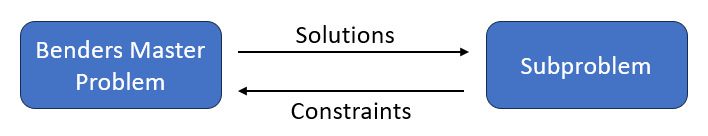
\includegraphics[width = 0.6\textwidth]{./images/BD.png}
  \end{figure}
\end{frame}

\begin{frame}{Obtain Seat Planning Composed of Full or Largest Patterns}
  % In most cases, we 

  There exists an optimal solution to SSP such that the patterns associated with this optimal solution are composed of the full or largest patterns under any given scenarios.

  \begin{description}
    \item[Step 1.] Obtain the solution, $\mathbf{x}^{*}$, by benders decomposition. Aggregate $\mathbf{x}^{*}$ to the number of each group type, ${s}_{i}^{0} =\sum_{j} x^{*}_{ij}, i \in \mathbf{M}$.

    \item[Step 2.] Solve problem \eqref{deter_upper} to obtain the optimal solution, $\mathbf{x}^{1}$. 
    % Aggregate $\mathbf{x}^{1}$ to the number of each group type, ${s}_{i}^{1} = \sum_{j} x^{1}_{ij}, i \in \mathbf{M}$.
     
    \item[Step 3.] Construct the full or largest patterns with $\mathbf{x}^{1}$.
 \end{description}
\end{frame}

% There exists an optimal solution to SSP such that the patterns associated with this optimal solution are composed of the full or largest patterns under any given scenarios.

% \begin{frame}{Issue of Optimality}
%   \begin{itemize}
%   \item In most cases, the optimal solution can be obtained.
%   \vspace{0.5cm}
%   \item For the extreme case where the optimal solution cannot be obtained, obtaining a feasible solution did not take too much time. 
%   \vspace{0.5cm}
%   \item It is more time-consuming to verify that it is the optimal solution. Thus, we set a time limit to obtain a feasible solution.
%   \vspace{0.5cm}
%   \item 
%   \end{itemize}
% \end{frame}


\begin{frame}{Running time of Benders Decomposition and IP}
  Parameters: 

  (150, 350): the demand of each group type is randomly sampled from (150, 350).

  (21, 50): the number of seats of each row is randomly sampled from (21, 50).
  \tiny
  \begin{table}[ht]
    \centering
    \begin{tabular}{|l|l|l|l|l|l|l|}
    \hline
    \# of scenarios & Demands & \# of rows & \# of groups & \# of seats & Running time of IP(s) & Benders (s) \\
    1000 & (20, 30) & 10 & 4 & (21, 30) & 1.6 & 0.1 \\
    1000 & (20, 30) & 10 & 4 & (21, 40) & 1.6 & 0.1 \\
    \hline
    1000  & (150, 350) & 30 & 8 & (21, 50) & 4.1  & 0.23 \\
    5000  &            &    &   &         & 28.73 & 0.47  \\
    10000 &            &    &   &         & 66.81  & 0.91 \\
    50000 &            &    &   &         & 925.17 & 4.3 \\
    \hline
    1000  & (1000, 2000) & 200 & 8 & (21, 50) & 5.88 & 0.29 \\
    5000  &              &     &   &          & 30.0 & 0.62 \\
    10000 &              &     &   &          & 64.41 & 1.09 \\
    50000 &              &     &   &          & 365.57 & 4.56\\
    \hline
    1000  & (150, 250) & 30 & 16 & (41, 60) & 17.15  & 0.18 \\
    5000  &            &    &    &          & 105.2  & 0.67 \\
    10000 &            &    &    &          & 260.88 & 1.28 \\
    50000 &            &    &    &          & 3873.16 & 6.18 \\
    \hline
    \end{tabular}
  \end{table}
\end{frame}
